\section{Promela-C-Integration}
\begin{figure}
  \centering
  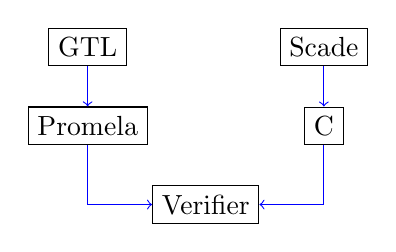
\begin{tikzpicture}
    \node[draw] (gtl) at (0,2) {GTL};
    \node[draw] (scade) at (3,2) {Scade};
    \node[draw] (promela) at (0,1) {Promela};
    \node[draw] (c) at (3,1) {C};
    \node[draw] (verifier) at (1.5,0) {Verifier};
    \draw[->,blue] (gtl) -- (promela);
    \draw[->,blue] (scade) -- (c);
    \draw[->,blue] (promela) |- (verifier);
    \draw[->,blue] (c) |- (verifier);
  \end{tikzpicture}
  \caption{Simulation durch C-Integration von Promela}
\end{figure}

Diese Übersetzungsmethode führt keine Optimierungen oder Abstraktionen durch, sondern simuliert das Modell exakt so, wie durch die Spezifikation angegeben.
Die Kontrakte für die synchronen Komponenten werden also ignoriert.

Zunächst wird jede synchrone Komponente mit Hilfe des SCADE-Compilers nach C übersetzt.
Dabei generiert der Compiler für jede Komponente zwei Datenstrukturen, die eine enthält die Eingabevariablen, die andere die Ausgabevariablen sowie den internen Zustand der Komponente.
Außerdem werden zwei Funktionen erstellt:
Die erste initialisiert den internen Zustand der Komponente, die zweite führt einen einzelnen Berechnungsschritt der Komponente durch.

Jede synchrone Komponente wird nun durch einen Promela-Prozess repräsentiert, der zunächst die Datenstrukturen initialisiert und dann in jedem Schritt die Eingabevariablen in die C-Datenstruktur kopiert, die Schrittfunktion aufruft und die Ergebnisse in die Ausgabevariablen schreibt.
